
\section{Introduction to DataStudio}

\textbf{Quick Reference Guide}

Shown below is the quick reference guide for DataStudio.

\vspace{0.3cm}
{\par\centering \resizebox*{0.95\textwidth}{!}{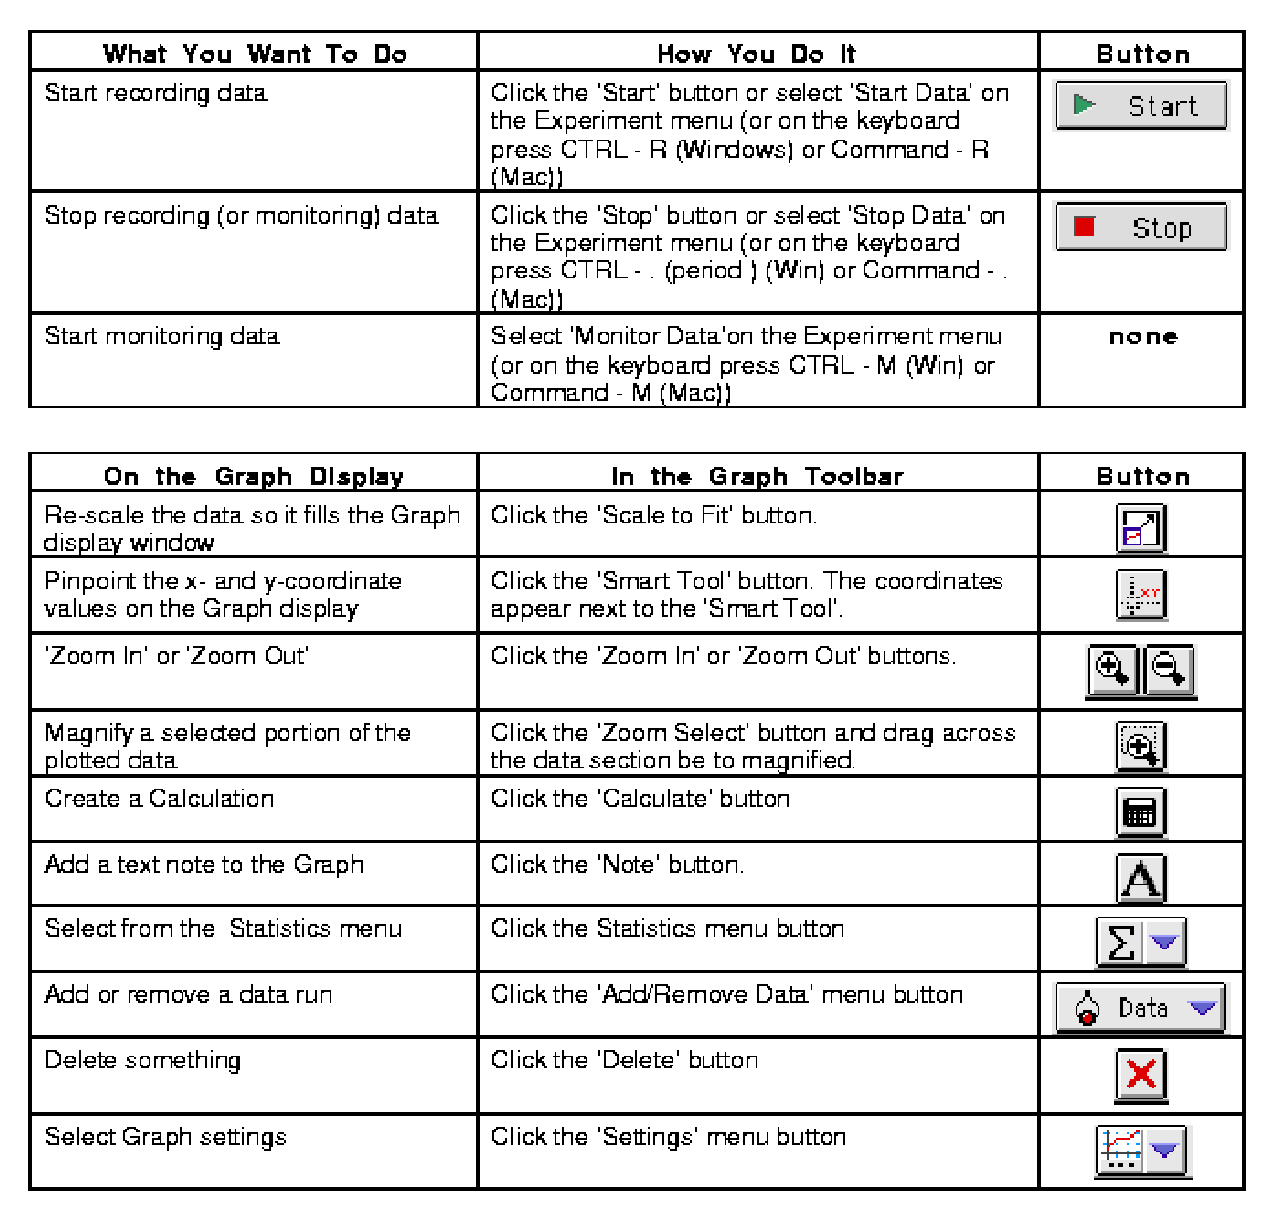
\includegraphics{appendices/datastudio/datastudio_fig1.eps}} \par}
\vspace{0.3cm}

\textbf{Selecting a Section of Data}

\begin{enumerate}
\item To select a data section, hold the mouse button down and move the cursor to
draw a rectangle around the data of interest. The data in the region of interest
will be highlighted.
\item To unselect the data, click anywhere in the graph window.
\end{enumerate}
\textbf{Fitting a Section of Data}

\begin{enumerate}
\item Select the section of data to be fitted.
\item Click on the \textbf{Fit} button on the Graph Toolbar and select a mathematical
model. The results of the fit will be displayed on the graph.
\item To remove the fit, click the \textbf{Fit} button and select the checked function
type.
\end{enumerate}
\textbf{Finding the Area Under a Curve}

\begin{enumerate}
\item Use the \textbf{Zoom Select} button on the Graph Toolbar to zoom in around the
region of interest in the graph. See the quick reference guide above for instructions.
\item Select the section of data that you want to integrate under.
\item Click the \textbf{Statistics} button on the Graph Toolbar and select \textbf{Area}.
The results of the integration will be displayed on the graph.
\item To undo the integration, click on the \textbf{Statistics} button and select
\textbf{Area}.
\end{enumerate}
